\documentclass[9pt,a4paper,landscape]{article}
\usepackage[utf8]{inputenc}
\usepackage[T1]{fontenc}
\usepackage[french]{babel}
\usepackage[margin=1cm,top=1.8cm,bottom=1.4cm]{geometry}
\usepackage{lmodern}
\usepackage{booktabs}
\usepackage{array}
\usepackage{longtable}
\usepackage{xcolor}
\usepackage{colortbl}
\usepackage{titlesec}
\usepackage{fancyhdr}
\usepackage{hyperref}
\usepackage{multicol}
\usepackage{amssymb}
\usepackage{tcolorbox}
\usepackage{tabularx}
\usepackage{setspace}
\usepackage{graphicx}
\usepackage{tikz}
\usepackage{enumitem}

% Couleurs
\definecolor{afblue}{RGB}{0,48,135}
\definecolor{afred}{RGB}{200,16,46}
\definecolor{afwhite}{RGB}{255,255,255}
\definecolor{aflight}{RGB}{220,230,245}
\definecolor{eurblue}{RGB}{0,51,153}
\definecolor{eurlight}{RGB}{235,242,255}
\definecolor{afrgreen}{RGB}{0,100,0}
\definecolor{afrlight}{RGB}{235,250,235}
\definecolor{asired}{RGB}{180,20,20}
\definecolor{asilight}{RGB}{255,238,238}
\definecolor{ameror}{RGB}{180,100,0}
\definecolor{amerlight}{RGB}{255,247,230}
\definecolor{mocolor}{RGB}{100,0,120}
\definecolor{molight}{RGB}{245,232,255}
\definecolor{omcolor}{RGB}{0,120,120}
\definecolor{omlight}{RGB}{225,248,248}
\definecolor{capgold}{RGB}{218,165,32}
\definecolor{darkbg}{RGB}{15,25,50}

% Section banners avec fond coloré
\newcommand{\sectionbanner}[2]{%
\noindent\colorbox{#1}{\parbox{\dimexpr\textwidth-2\fboxsep}{%
\vspace{3pt}\hspace{6pt}{\Large\bfseries\color{white}#2}\vspace{3pt}}}%
\vspace{4pt}%
}

% Style titres (pour subsections only)
\titleformat{\section}{\Large\bfseries\color{afblue}}{}{0em}{}
\titleformat{\subsection}{\normalsize\bfseries}{}{0em}{}
\titlespacing{\section}{0pt}{6pt}{3pt}
\titlespacing{\subsection}{0pt}{3pt}{2pt}

% Header avec bande tricolore
\pagestyle{fancy}
\fancyhf{}
\fancyhead[L]{\small\color{afblue}\textbf{DESTINATIONS --- GROUPE AIR FRANCE 2025/2026}}
\fancyhead[R]{\small\color{afblue}\textit{PSY0 Cadets Air France}}
\fancyfoot[C]{%
\begin{tikzpicture}[baseline=0pt]
\fill[afblue] (0,0) rectangle (3,2pt);
\fill[white] (3,0) rectangle (6,2pt);
\fill[afred] (6,0) rectangle (9,2pt);
\end{tikzpicture}\\[-4pt]
{\footnotesize\color{afblue}\thepage}%
}
\renewcommand{\headrulewidth}{2pt}
\renewcommand{\headrule}{\hbox to\headwidth{\color{afblue}\leaders\hrule height \headrulewidth\hfill}}
\setlength{\headheight}{16pt}
\setlength{\footskip}{20pt}

\hypersetup{colorlinks=true,linkcolor=afblue,urlcolor=afblue}
\setlength{\parindent}{0pt}
\setlength{\tabcolsep}{3pt}
\renewcommand{\arraystretch}{1.08}

% Commande capitale
\newcommand{\CAP}{\textcolor{capgold}{$\bigstar$}}

\begin{document}

% ==================== PAGE DE COUVERTURE ====================
\thispagestyle{empty}
\newgeometry{margin=0pt}
\noindent\begin{tikzpicture}[remember picture,overlay]
% Fond bleu foncé
\fill[darkbg] (current page.south west) rectangle (current page.north east);
% Image de couverture
\node[anchor=center,inner sep=0pt] at ([yshift=2cm]current page.center) {%
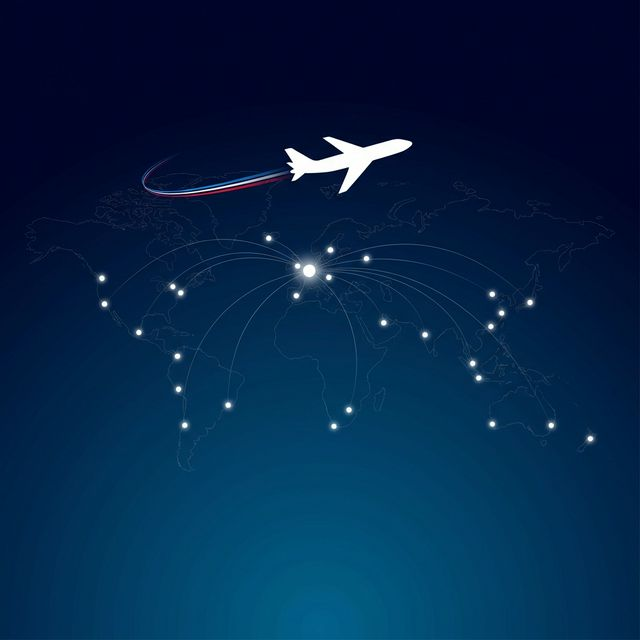
\includegraphics[width=0.55\paperwidth]{cover_banner.png}};
% Titre
\node[anchor=center,text=white] at ([yshift=-3cm]current page.center) {%
\begin{minipage}{0.8\paperwidth}\centering
{\fontsize{36}{42}\selectfont\bfseries DESTINATIONS}\\[0.4cm]
{\fontsize{20}{26}\selectfont GROUPE AIR FRANCE}\\[0.6cm]
\textcolor{afblue}{\rule{4cm}{3pt}}\textcolor{white}{\rule{4cm}{3pt}}\textcolor{afred}{\rule{4cm}{3pt}}\\[0.6cm]
{\Large Air France $\bullet$ Transavia France $\bullet$ Air France HOP}\\[0.3cm]
{\large $\sim$200 destinations $\bullet$ $\sim$80 pays $\bullet$ Saison 2025/2026}\\[0.5cm]
{\normalsize Document de révision --- PSY0 Cadets Air France}
\end{minipage}};
\end{tikzpicture}
\clearpage
\restoregeometry

% ==================== TABLE DES MATIÈRES ====================
\thispagestyle{fancy}
\sectionbanner{afblue}{TABLE DES MATIÈRES}
\vspace{0.2cm}
\begin{multicols}{3}
\small
\tableofcontents
\end{multicols}

\vspace{0.4cm}
\begin{tcolorbox}[colback=aflight,colframe=afblue,boxrule=1.5pt,arc=4pt]
\centering\small
\CAP\ = Capitale du pays \quad\textbf{|}\quad \textbf{Dist.} = distance depuis Paris (km) \quad\textbf{|}\quad \textbf{Vol} = durée approximative \quad\textbf{|}\quad \textbf{UTC} = fuseau horaire\\[2pt]
\textbf{AF} = Air France \quad\textbf{|}\quad \textbf{TO} = Transavia France \quad\textbf{|}\quad \textbf{HOP} = Air France HOP
\end{tcolorbox}
\vspace{-0.2cm}

% ===================== FRANCE =========================
\sectionbanner{afblue}{\texorpdfstring{$\bigstar$}{} FRANCE MÉTROPOLITAINE}
\addcontentsline{toc}{section}{France Métropolitaine}

\noindent
\begin{minipage}[t]{0.48\textwidth}
\scriptsize
\begin{tabular}{@{}l c c c@{}}
\toprule
\textbf{Ville} & \textbf{IATA} & \textbf{OACI} & \textbf{Cie} \\
\midrule
\rowcolor{aflight}\CAP\ Paris CDG & CDG & LFPG & AF \\
\CAP\ Paris Orly & ORY & LFPO & AF/TO \\
\rowcolor{aflight} Ajaccio & AJA & LFKJ & AF/TO \\
Bastia & BIA & LFKB & AF/TO \\
\rowcolor{aflight} Biarritz & BIQ & LFBZ & AF \\
Bordeaux & BOD & LFBD & AF/TO \\
\rowcolor{aflight} Brest & BES & LFRB & AF \\
Caen & CFR & LFRK & HOP \\
\rowcolor{aflight} Calvi & CLY & LFKC & AF/TO \\
Clermont-Fd & CFE & LFLC & AF \\
\rowcolor{aflight} Figari & FSC & LFKF & AF/TO \\
Grenoble & GNB & LFLS & TO \\
\rowcolor{aflight} Lille & LIL & LFQQ & TO \\
\bottomrule
\end{tabular}
\end{minipage}\hfill
\begin{minipage}[t]{0.48\textwidth}
\scriptsize
\begin{tabular}{@{}l c c c@{}}
\toprule
\textbf{Ville} & \textbf{IATA} & \textbf{OACI} & \textbf{Cie} \\
\midrule
\rowcolor{aflight} Lyon & LYS & LFLL & AF/TO \\
Marseille & MRS & LFML & AF/TO \\
\rowcolor{aflight} Montpellier & MPL & LFMT & AF/TO \\
Nantes & NTE & LFRS & AF/TO \\
\rowcolor{aflight} Nice & NCE & LFMN & AF/TO \\
Pau & PUF & LFBP & AF \\
\rowcolor{aflight} Perpignan & PGF & LFMP & TO \\
Rennes & RNS & LFRN & AF \\
\rowcolor{aflight} Strasbourg & SXB & LFST & HOP \\
Toulon & TLN & LFTH & TO \\
\rowcolor{aflight} Toulouse & TLS & LFBO & AF/TO \\
Bergerac & EGC & LFBE & TO \\
\bottomrule
\end{tabular}
\end{minipage}

% ===================== EUROPE =========================
\sectionbanner{eurblue}{EUROPE --- $\sim$116 destinations, 27 pays}
\addcontentsline{toc}{section}{Europe (116 destinations)}

\begin{multicols}{3}
\scriptsize

\textbf{\color{eurblue}ALLEMAGNE}\\[-0.1cm]
\begin{tabular}{@{}l c c c c c@{}}
\toprule
\textbf{Ville} & \textbf{IATA} & \textbf{OACI} & \textbf{Dist} & \textbf{Vol} & \textbf{Cie} \\
\midrule
\rowcolor{eurlight}\CAP\ Berlin & BER & EDDB & 878 & 1h50 & AF \\
Düsseldorf & DUS & EDDL & 407 & 1h15 & AF \\
\rowcolor{eurlight} Francfort & FRA & EDDF & 479 & 1h20 & AF \\
Hambourg & HAM & EDDH & 740 & 1h40 & AF \\
\rowcolor{eurlight} Munich & MUC & EDDM & 685 & 1h30 & AF \\
Stuttgart & STR & EDDS & 504 & 1h20 & AF \\
\bottomrule
\end{tabular}

\vspace{0.15cm}
\textbf{\color{eurblue}ESPAGNE}\\[-0.1cm]
\begin{tabular}{@{}l c c c c c@{}}
\toprule
\textbf{Ville} & \textbf{IATA} & \textbf{OACI} & \textbf{Dist} & \textbf{Vol} & \textbf{Cie} \\
\midrule
\rowcolor{eurlight}\CAP\ Madrid & MAD & LEMD & 1054 & 2h10 & AF/TO \\
Alicante & ALC & LEAL & 1099 & 2h10 & TO \\
\rowcolor{eurlight} Barcelone & BCN & LEBL & 831 & 1h50 & AF/TO \\
Bilbao & BIO & LEBB & 776 & 1h35 & TO \\
\rowcolor{eurlight} Fuerteventura & FUE & GCFV & 2879 & 4h15 & TO \\
Gran Canaria & LPA & GCLP & 2855 & 4h10 & TO \\
\rowcolor{eurlight} Ibiza & IBZ & LEIB & 1094 & 2h00 & AF/TO \\
Lanzarote & ACE & GCRR & 2907 & 4h15 & TO \\
\rowcolor{eurlight} Malaga & AGP & LEMG & 1389 & 2h30 & AF/TO \\
Majorque & PMI & LEPA & 1041 & 2h00 & AF/TO \\
\rowcolor{eurlight} Minorque & MAH & LEMH & 1065 & 1h55 & TO \\
Séville & SVQ & LEZL & 1321 & 2h25 & AF/TO \\
\rowcolor{eurlight} Tenerife & TFS & GCTS & 2874 & 4h20 & AF/TO \\
Valence & VLC & LEVC & 1034 & 2h00 & AF/TO \\
\bottomrule
\end{tabular}

\vspace{0.15cm}
\textbf{\color{eurblue}ITALIE}\\[-0.1cm]
\begin{tabular}{@{}l c c c c c@{}}
\toprule
\textbf{Ville} & \textbf{IATA} & \textbf{OACI} & \textbf{Dist} & \textbf{Vol} & \textbf{Cie} \\
\midrule
\rowcolor{eurlight}\CAP\ Rome & FCO & LIRF & 1106 & 2h10 & AF/TO \\
Bari & BRI & LIBD & 1360 & 2h20 & AF/TO \\
\rowcolor{eurlight} Bologne & BLQ & LIPE & 860 & 1h45 & AF/TO \\
Brindisi & BDS & LIBR & 1490 & 2h30 & TO \\
\rowcolor{eurlight} Cagliari & CAG & LIEE & 1250 & 1h55 & AF/TO \\
Catane & CTA & LICC & 1570 & 2h35 & AF/TO \\
\rowcolor{eurlight} Florence & FLR & LIRQ & 890 & 1h50 & AF \\
Milan Lin. & LIN & LIML & 640 & 1h25 & AF \\
\rowcolor{eurlight} Milan Malp. & MXP & LIMC & 640 & 1h25 & AF/TO \\
Naples & NAP & LIRN & 1260 & 2h15 & AF/TO \\
\rowcolor{eurlight} Olbia & OLB & LIEO & 1090 & 1h45 & AF/TO \\
Palerme & PMO & LICJ & 1430 & 2h25 & AF/TO \\
\rowcolor{eurlight} Pise & PSA & LIRP & 880 & 1h45 & TO \\
Venise & VCE & LIPZ & 840 & 1h40 & AF/TO \\
\rowcolor{eurlight} Vérone & VRN & LIPX & 750 & 1h35 & AF \\
\bottomrule
\end{tabular}

\vspace{0.15cm}
\textbf{\color{eurblue}GRÈCE}\\[-0.1cm]
\begin{tabular}{@{}l c c c c c@{}}
\toprule
\textbf{Ville} & \textbf{IATA} & \textbf{OACI} & \textbf{Dist} & \textbf{Vol} & \textbf{Cie} \\
\midrule
\rowcolor{eurlight}\CAP\ Athènes & ATH & LGAV & 2095 & 3h20 & AF/TO \\
Corfou & CFU & LGKR & 1620 & 2h40 & TO \\
\rowcolor{eurlight} Héraklion & HER & LGIR & 2395 & 3h30 & AF/TO \\
Kos & KGS & LGKO & 2460 & 3h25 & TO \\
\rowcolor{eurlight} Mykonos & JMK & LGMK & 2280 & 3h20 & AF/TO \\
Rhodes & RHO & LGRP & 2560 & 3h30 & AF/TO \\
\rowcolor{eurlight} Santorin & JTR & LGSR & 2370 & 3h25 & AF/TO \\
Thessalonique & SKG & LGTS & 1840 & 2h50 & AF/TO \\
\rowcolor{eurlight} Zakynthos & ZTH & LGZA & 1730 & 2h50 & TO\\
\bottomrule
\end{tabular}

\vspace{0.15cm}
\textbf{\color{eurblue}PORTUGAL}\\[-0.1cm]
\begin{tabular}{@{}l c c c c c@{}}
\toprule
\rowcolor{eurlight}\CAP\ Lisbonne & LIS & LPPT & 1454 & 2h35 & AF/TO \\
Faro & FAO & LPFR & 1594 & 2h45 & AF/TO \\
\rowcolor{eurlight} Funchal (Mad.) & FNC & LPMA & 2383 & 3h40 & TO \\
Porto & OPO & LPPR & 1185 & 2h15 & AF/TO \\
\bottomrule
\end{tabular}

\vspace{0.15cm}
\textbf{\color{eurblue}ROYAUME-UNI}\\[-0.1cm]
\begin{tabular}{@{}l c c c c c@{}}
\toprule
\rowcolor{eurlight}\CAP\ Londres LHR & LHR & EGLL & 340 & 1h15 & AF \\
Londres City & LCY & EGLC & 340 & 1h15 & AF \\
\rowcolor{eurlight} Édimbourg & EDI & EGPH & 870 & 1h50 & AF/TO \\
Exeter & EXT & EGTE & 400 & 1h15 & AF \\
\rowcolor{eurlight} Manchester & MAN & EGCC & 570 & 1h30 & AF \\
\bottomrule
\end{tabular}

\vspace{0.15cm}
\textbf{\color{eurblue}SCANDINAVIE \& BALTIQUE}\\[-0.1cm]
\begin{tabular}{@{}l l c c c c c@{}}
\toprule
\textbf{Pays} & \textbf{Ville} & \textbf{IATA} & \textbf{OACI} & \textbf{Dist} & \textbf{Vol} & \textbf{Cie} \\
\midrule
\rowcolor{eurlight} Danemark & \CAP\ Copenhague & CPH & EKCH & 1025 & 2h & AF/TO \\
Finlande & \CAP\ Helsinki & HEL & EFHK & 1910 & 2h55 & AF \\
\rowcolor{eurlight} Norvège & \CAP\ Oslo & OSL & ENGM & 1344 & 2h15 & AF/TO \\
Suède & \CAP\ Stockholm & ARN & ESSA & 1540 & 2h30 & AF \\
\rowcolor{eurlight} Estonie & \CAP\ Tallinn & TLL & EETN & 1870 & 2h50 & TO \\
Lettonie & \CAP\ Riga & RIX & EVRA & 1660 & 2h40 & TO \\
\rowcolor{eurlight} Finlande & Kittilä & KTT & EFKT & 2750 & 3h50 & AF/TO \\
Suède & Kiruna & KRN & ESNQ & 2580 & 3h40 & AF \\
\rowcolor{eurlight} Finlande & Rovaniemi & RVN & EFRO & 2660 & 3h45 & AF/TO \\
Norvège & Tromsø & TOS & ENTC & 2660 & 3h45 & AF \\
\bottomrule
\end{tabular}

\vspace{0.15cm}
\textbf{\color{eurblue}EUROPE CENTRALE \& EST}\\[-0.1cm]
\begin{tabular}{@{}l l c c c c c@{}}
\toprule
\textbf{Pays} & \textbf{Ville} & \textbf{IATA} & \textbf{OACI} & \textbf{Dist} & \textbf{Vol} & \textbf{Cie} \\
\midrule
\rowcolor{eurlight} Serbie & \CAP\ Belgrade & BEG & LYBE & 1425 & 2h25 & AF/TO \\
Roumanie & \CAP\ Bucarest & OTP & LROP & 1860 & 3h & AF \\
\rowcolor{eurlight} Hongrie & \CAP\ Budapest & BUD & LHBP & 1240 & 2h10 & AF \\
Slovénie & \CAP\ Ljubljana & LJU & LJLJ & 895 & 1h45 & AF \\
\rowcolor{eurlight} Tchéquie & \CAP\ Prague & PRG & LKPR & 878 & 1h45 & AF/TO \\
Bulgarie & \CAP\ Sofia & SOF & LBSF & 1750 & 2h45 & TO \\
\rowcolor{eurlight} Albanie & \CAP\ Tirana & TIA & LATI & 1530 & 2h30 & AF/TO \\
Pologne & \CAP\ Varsovie & WAW & EPWA & 1370 & 2h15 & AF \\
\rowcolor{eurlight} Autriche & \CAP\ Vienne & VIE & LOWW & 1034 & 2h & AF/TO \\
Croatie & \CAP\ Zagreb & ZAG & LDZA & 1070 & 1h55 & AF \\
\rowcolor{eurlight} Pologne & Cracovie & KRK & EPKK & 1290 & 2h10 & AF \\
Bosnie-H. & Sarajevo & SJJ & LQSA & 1370 & 2h20 & TO \\
\bottomrule
\end{tabular}

\vspace{0.15cm}
\textbf{\color{eurblue}AUTRE EUROPE}\\[-0.1cm]
\begin{tabular}{@{}l l c c c c c@{}}
\toprule
\textbf{Pays} & \textbf{Ville} & \textbf{IATA} & \textbf{OACI} & \textbf{Dist} & \textbf{Vol} & \textbf{Cie} \\
\midrule
\rowcolor{eurlight} Pays-Bas & \CAP\ Amsterdam & AMS & EHAM & 430 & 1h15 & AF \\
Belgique & \CAP\ Bruxelles & BRU & EBBR & 264 & 1h05 & AF/TO \\
\rowcolor{eurlight} Irlande & \CAP\ Dublin & DUB & EIDW & 782 & 1h40 & AF \\
Suisse & Genève & GVA & LSGG & 405 & 1h10 & AF/TO \\
\rowcolor{eurlight} Malte & \CAP\ La Valette & MLA & LMML & 1665 & 2h40 & AF/TO \\
Islande & \CAP\ Reykjavik & KEF & BIKF & 2418 & 3h50 & AF/TO \\
\rowcolor{eurlight} Irlande & Cork & ORK & EICK & 895 & 1h50 & AF \\
Suisse & Zürich & ZRH & LSZH & 490 & 1h15 & AF \\
\rowcolor{eurlight} Turquie & \CAP\ Istanbul & IST & LTFM & 2240 & 3h30 & AF \\
Turquie & Antalya & AYT & LTAI & 2690 & 3h45 & TO \\
\rowcolor{eurlight} Croatie & Dubrovnik & DBV & LDDU & 1370 & 2h15 & AF/TO \\
Croatie & Split & SPU & LDSP & 1260 & 2h10 & AF/TO \\
\rowcolor{eurlight} Montén. & Tivat & TIV & LYTV & 1420 & 2h20 & TO \\
Autriche & Innsbruck & INN & LOWI & 745 & 1h30 & TO \\
\rowcolor{eurlight} Autriche & Salzbourg & SZG & LOWS & 800 & 1h35 & TO \\
Chypre & Larnaca & LCA & LCLK & 2910 & 4h10 & TO \\
\bottomrule
\end{tabular}
\end{multicols}

% ===================== AFRIQUE DU NORD ================
\sectionbanner{afrgreen}{AFRIQUE DU NORD}
\addcontentsline{toc}{section}{Afrique du Nord}

\begin{multicols}{3}
\scriptsize

\textbf{\color{afrgreen}MAROC} \textit{(UTC+1)}\\[-0.1cm]
\begin{tabular}{@{}l c c c c c@{}}
\toprule
\textbf{Ville} & \textbf{IATA} & \textbf{OACI} & \textbf{Dist} & \textbf{Vol} & \textbf{Cie} \\
\midrule
\rowcolor{afrlight}\CAP\ Rabat & RBA & GMME & 1636 & 2h50 & AF \\
Agadir & AGA & GMAD & 2309 & 3h30 & AF/TO \\
\rowcolor{afrlight} Casablanca & CMN & GMMN & 1875 & 3h05 & AF/TO \\
Essaouira & ESU & GMMI & 2190 & 3h20 & TO \\
\rowcolor{afrlight} Fès & FEZ & GMFF & 1720 & 2h55 & AF/TO \\
Marrakech & RAK & GMMX & 2108 & 3h25 & AF/TO \\
\rowcolor{afrlight} Nador & NDR & GMMW & 1530 & 2h40 & AF/TO \\
Oujda & OUD & GMFO & 1518 & 2h35 & AF/TO \\
\rowcolor{afrlight} Tanger & TNG & GMTT & 1559 & 2h40 & AF/TO \\
\bottomrule
\end{tabular}

\vspace{0.15cm}
\textbf{\color{afrgreen}ALGÉRIE} \textit{(UTC+1)}\\[-0.1cm]
\begin{tabular}{@{}l c c c c c@{}}
\toprule
\rowcolor{afrlight}\CAP\ Alger & ALG & DAAG & 1344 & 2h20 & AF/TO \\
Annaba & AAE & DABB & 1365 & 2h15 & TO \\
\rowcolor{afrlight} Béjaïa & BJA & DAAE & 1345 & 2h15 & TO \\
Constantine & CZL & DABC & 1430 & 2h25 & TO \\
\rowcolor{afrlight} Oran & ORN & DAOO & 1326 & 2h20 & AF/TO \\
Sétif & QSF & DAAS & 1400 & 2h20 & TO \\
\rowcolor{afrlight} Tlemcen & TLM & DAON & 1400 & 2h25 & TO \\
\bottomrule
\end{tabular}

\vspace{0.15cm}
\textbf{\color{afrgreen}TUNISIE} \textit{(UTC+1)}\\[-0.1cm]
\begin{tabular}{@{}l c c c c c@{}}
\toprule
\rowcolor{afrlight}\CAP\ Tunis & TUN & DTTA & 1497 & 2h30 & AF/TO \\
Djerba & DJE & DTTJ & 1740 & 2h45 & TO \\
\rowcolor{afrlight} Monastir & MIR & DTMB & 1620 & 2h35 & TO \\
\bottomrule
\end{tabular}

\vspace{0.15cm}
\textbf{\color{afrgreen}ÉGYPTE} \textit{(UTC+2)}\\[-0.1cm]
\begin{tabular}{@{}l c c c c c@{}}
\toprule
\rowcolor{afrlight}\CAP\ Le Caire & CAI & HECA & 3210 & 4h30 & AF \\
Hurghada & HRG & HEGN & 3800 & 5h00 & TO \\
\bottomrule
\end{tabular}

\end{multicols}

% =========== AFRIQUE SUBSAHARIENNE ====================
\sectionbanner{afrgreen}{AFRIQUE SUBSAHARIENNE --- $\sim$28 destinations, 22 pays}
\addcontentsline{toc}{section}{Afrique Subsaharienne}

\begin{multicols}{3}
\scriptsize

\textbf{\color{afrgreen}AFRIQUE DE L'OUEST}\\[-0.1cm]
\begin{tabular}{@{}l c c c c c@{}}
\toprule
\textbf{Pays} & \textbf{Ville} & \textbf{IATA} & \textbf{OACI} & \textbf{Vol} & \textbf{UTC} \\
\midrule
\rowcolor{afrlight} Bénin & Cotonou & COO & DBBB & 6h20 & +1 \\
Côte Iv. & \CAP\ Abidjan & ABJ & DIAP & 6h25 & 0 \\
\rowcolor{afrlight} Ghana & \CAP\ Accra & ACC & DGAA & 6h20 & 0 \\
Guinée & \CAP\ Conakry & CKY & GUCY & 6h15 & 0 \\
\rowcolor{afrlight} G. Éq. & \CAP\ Malabo & SSG & FGSL & 6h10 & +1 \\
Maurice & \CAP\ Nouakch. & NKC & GQNN & 5h30 & 0 \\
\rowcolor{afrlight} Niger & \CAP\ Niamey & NIM & DRRN & 5h40 & +1 \\
Nigéria & \CAP\ Abuja & ABV & DNAA & 6h10 & +1 \\
\rowcolor{afrlight} Nigéria & Lagos & LOS & DNMM & 6h30 & +1 \\
Sénégal & \CAP\ Dakar & DSS & GOBD & 5h45 & 0 \\
\rowcolor{afrlight} Togo & \CAP\ Lomé & LFW & DXXX & 6h25 & 0 \\
\bottomrule
\end{tabular}

\vspace{0.15cm}
\textbf{\color{afrgreen}AFRIQUE CENTRALE}\\[-0.1cm]
\begin{tabular}{@{}l c c c c c@{}}
\toprule
\rowcolor{afrlight} Cameroun & \CAP\ Yaoundé & NSI & FKYS & 6h10 & +1 \\
Cameroun & Douala & DLA & FKKD & 6h15 & +1 \\
\rowcolor{afrlight} Congo & \CAP\ Brazzaville & BZV & FCBB & 7h40 & +1 \\
Congo & Pointe-N. & PNR & FCPP & 7h20 & +1 \\
\rowcolor{afrlight} Gabon & \CAP\ Libreville & LBV & FOOL & 6h45 & +1 \\
RCA & \CAP\ Bangui & BGF & FEFF & 6h45 & +1 \\
\rowcolor{afrlight} RDC & \CAP\ Kinshasa & FIH & FZAA & 7h50 & +1 \\
Tchad & \CAP\ N'Djamena & NDJ & FTTJ & 5h50 & +1 \\
\bottomrule
\end{tabular}

\vspace{0.15cm}
\textbf{\color{afrgreen}AFRIQUE DE L'EST \& SUD}\\[-0.1cm]
\begin{tabular}{@{}l c c c c c@{}}
\toprule
\rowcolor{afrlight} Afr. Sud & Johannesb. & JNB & FAOR & 10h30 & +2 \\
Afr. Sud & Le Cap & CPT & FACT & 11h30 & +2 \\
\rowcolor{afrlight} Angola & \CAP\ Luanda & LAD & FNLU & 8h00 & +1 \\
Djibouti & \CAP\ Djibouti & JIB & HDAM & 6h00 & +3 \\
\rowcolor{afrlight} Kenya & \CAP\ Nairobi & NBO & HKJK & 8h30 & +3 \\
Ouganda & \CAP\ Kampala & EBB & HUEN & 8h15 & +3 \\
\rowcolor{afrlight} Rwanda & \CAP\ Kigali & KGL & HRYR & 8h35 & +2 \\
Tanzanie & \CAP\ Dar es S. & DAR & HTDA & 9h40 & +3 \\
\rowcolor{afrlight} Tanzanie & Kilimandjaro & JRO & HTKJ & 9h00 & +3 \\
Tanzanie & Zanzibar & ZNZ & HTZA & 9h50 & +3 \\
\rowcolor{afrlight} Madagas. & \CAP\ Antanan. & TNR & FMMI & 11h00 & +3 \\
Madagas. & Nosy Be & NOS & FMNN & 10h30 & +3 \\
\bottomrule
\end{tabular}

\end{multicols}

% =========== OCÉAN INDIEN ============================
\sectionbanner{omcolor}{OCÉAN INDIEN}
\addcontentsline{toc}{section}{Océan Indien}

\begin{center}
\scriptsize
\begin{tabular}{@{}l l c c c c c@{}}
\toprule
\textbf{Territ./Pays} & \textbf{Ville} & \textbf{IATA} & \textbf{OACI} & \textbf{Vol} & \textbf{UTC} & \textbf{Cie} \\
\midrule
\rowcolor{omlight} Île Maurice & \CAP\ Port Louis & MRU & FIMP & 11h15 & +4 & AF \\
La Réunion (FR) & Saint-Denis & RUN & FMEE & 11h00 & +4 & AF \\
\rowcolor{omlight} Mayotte (FR) & Dzaoudzi & DZA & FMCZ & 10h30 & +3 & AF \\
Maldives & \CAP\ Malé & MLE & VRMM & 10h00 & +5 & AF \\
\bottomrule
\end{tabular}
\end{center}

% =========== MOYEN-ORIENT ============================
\sectionbanner{mocolor}{MOYEN-ORIENT}
\addcontentsline{toc}{section}{Moyen-Orient}

\begin{center}
\scriptsize
\begin{tabular}{@{}l l c c c c c@{}}
\toprule
\textbf{Pays} & \textbf{Ville} & \textbf{IATA} & \textbf{OACI} & \textbf{Vol} & \textbf{UTC} & \textbf{Cie} \\
\midrule
\rowcolor{molight} Arabie S. & \CAP\ Riyad & RUH & OERK & 6h00 & +3 & AF \\
Arabie S. & Djeddah & JED & OEJN & 5h30 & +3 & AF/TO \\
\rowcolor{molight} Bahreïn & \CAP\ Manama & BAH & OBBI & 6h15 & +3 & AF \\
EAU & \CAP\ Abu Dhabi & AUH & OMAA & 6h40 & +4 & AF \\
\rowcolor{molight} EAU & Dubaï & DXB & OMDB & 6h30 & +4 & AF/TO \\
Israël & Tel Aviv & TLV & LLBG & 4h30 & +2 & AF/TO \\
\rowcolor{molight} Jordanie & \CAP\ Amman & AMM & OJAI & 4h20 & +3 & TO \\
Liban & \CAP\ Beyrouth & BEY & OLBA & 4h15 & +2 & AF \\
\bottomrule
\end{tabular}
\end{center}

% ============ ASIE-PACIFIQUE ==========================
\sectionbanner{asired}{ASIE-PACIFIQUE}
\addcontentsline{toc}{section}{Asie-Pacifique}

\begin{multicols}{2}
\scriptsize
\begin{tabular}{@{}l l c c c c c@{}}
\toprule
\textbf{Pays} & \textbf{Ville} & \textbf{IATA} & \textbf{OACI} & \textbf{Vol} & \textbf{UTC} & \textbf{Cie} \\
\midrule
\rowcolor{asilight} Chine & \CAP\ Pékin & PEK & ZBAA & 10h & +8 & AF \\
Chine & Shanghai & PVG & ZSPD & 11h30 & +8 & AF \\
\rowcolor{asilight} Chine & Hong Kong & HKG & VHHH & 11h30 & +8 & AF \\
Corée S. & \CAP\ Séoul & ICN & RKSI & 11h & +9 & AF \\
\rowcolor{asilight} Inde & \CAP\ New Delhi & DEL & VIDP & 8h15 & +5:30 & AF \\
Inde & Mumbai & BOM & VABB & 9h & +5:30 & AF \\
\rowcolor{asilight} Japon & \CAP\ Tokyo HND & HND & RJTT & 12h & +9 & AF \\
Japon & Tokyo NRT & NRT & RJAA & 12h & +9 & AF \\
\bottomrule
\end{tabular}

\columnbreak

\begin{tabular}{@{}l l c c c c c@{}}
\toprule
\textbf{Pays} & \textbf{Ville} & \textbf{IATA} & \textbf{OACI} & \textbf{Vol} & \textbf{UTC} & \textbf{Cie} \\
\midrule
\rowcolor{asilight} Japon & Osaka & KIX & RJBB & 12h & +9 & AF \\
Philippines & \CAP\ Manille & MNL & RPLL & 13h & +8 & AF \\
\rowcolor{asilight} Singapour & \CAP\ Singapour & SIN & WSSS & 12h30 & +8 & AF \\
Thaïlande & \CAP\ Bangkok & BKK & VTBS & 11h15 & +7 & AF \\
\rowcolor{asilight} Thaïlande & Phuket & HKT & VTSP & 11h30 & +7 & AF \\
Vietnam & Hô Chi Minh & SGN & VVTS & 12h & +7 & AF \\
\rowcolor{asilight} Arménie & \CAP\ Erevan & EVN & UDYZ & 4h30 & +4 & TO \\
Cap-Vert & Boa Vista & BVC & GVBA & 5h50 & $-$1 & TO \\
\bottomrule
\end{tabular}
\end{multicols}

% ============ AMÉRIQUES ==============================
\sectionbanner{ameror}{AMÉRIQUES}
\addcontentsline{toc}{section}{Amériques}

\begin{multicols}{2}
\scriptsize

\textbf{\color{ameror}ÉTATS-UNIS} \textit{(19 dest.)}\\[-0.1cm]
\begin{tabular}{@{}l c c c c c@{}}
\toprule
\textbf{Ville} & \textbf{IATA} & \textbf{OACI} & \textbf{Vol} & \textbf{UTC} & \textbf{Cie} \\
\midrule
\rowcolor{amerlight}\CAP\ Washington & IAD & KIAD & 8h30 & $-$5 & AF \\
Atlanta & ATL & KATL & 9h30 & $-$5 & AF \\
\rowcolor{amerlight} Boston & BOS & KBOS & 7h30 & $-$5 & AF \\
Chicago & ORD & KORD & 9h & $-$6 & AF \\
\rowcolor{amerlight} Dallas & DFW & KDFW & 10h15 & $-$6 & AF \\
Denver & DEN & KDEN & 10h & $-$7 & AF \\
\rowcolor{amerlight} Détroit & DTW & KDTW & 8h45 & $-$5 & AF \\
Houston & IAH & KIAH & 10h30 & $-$6 & AF \\
\rowcolor{amerlight} Las Vegas & LAS & KLAS & 11h15 & $-$8 & AF \\
Los Angeles & LAX & KLAX & 11h15 & $-$8 & AF \\
\rowcolor{amerlight} Miami & MIA & KMIA & 9h45 & $-$5 & AF \\
Minneapolis & MSP & KMSP & 9h15 & $-$6 & AF \\
\rowcolor{amerlight} New York JFK & JFK & KJFK & 8h15 & $-$5 & AF \\
Newark & EWR & KEWR & 8h15 & $-$5 & AF \\
\rowcolor{amerlight} Orlando & MCO & KMCO & 9h45 & $-$5 & AF \\
Phoenix & PHX & KPHX & 11h & $-$7 & AF \\
\rowcolor{amerlight} Raleigh-Durh. & RDU & KRDU & 9h & $-$5 & AF \\
San Francisco & SFO & KSFO & 11h30 & $-$8 & AF \\
\rowcolor{amerlight} Seattle & SEA & KSEA & 10h30 & $-$8 & AF \\
\bottomrule
\end{tabular}

\columnbreak

\textbf{\color{ameror}CANADA} \textit{(5 dest.)}\\[-0.1cm]
\begin{tabular}{@{}l c c c c c@{}}
\toprule
\rowcolor{amerlight}\CAP\ Ottawa & YOW & CYOW & 7h30 & $-$5 & AF \\
Montréal & YUL & CYUL & 7h30 & $-$5 & AF \\
\rowcolor{amerlight} Québec & YQB & CYQB & 7h15 & $-$5 & AF \\
Toronto & YYZ & CYYZ & 8h & $-$5 & AF \\
\rowcolor{amerlight} Vancouver & YVR & CYVR & 10h & $-$8 & AF \\
\bottomrule
\end{tabular}

\vspace{0.15cm}
\textbf{\color{ameror}MEXIQUE \& AM. CENTRALE}\\[-0.1cm]
\begin{tabular}{@{}l c c c c c@{}}
\toprule
\rowcolor{amerlight}\CAP\ Mexico & MEX & MMMX & 11h30 & $-$6 & AF \\
Cancún & CUN & MMUN & 10h30 & $-$5 & AF/TO \\
\rowcolor{amerlight}\CAP\ San José (CR) & SJO & MROC & 11h & $-$6 & AF \\
\bottomrule
\end{tabular}

\vspace{0.15cm}
\textbf{\color{ameror}AMÉRIQUE DU SUD}\\[-0.1cm]
\begin{tabular}{@{}l c c c c c@{}}
\toprule
\rowcolor{amerlight}\CAP\ Buenos Aires & EZE & SAEZ & 13h30 & $-$3 & AF \\
\CAP\ Bogota & BOG & SKBO & 10h45 & $-$5 & AF \\
\rowcolor{amerlight}\CAP\ Lima & LIM & SPJC & 12h30 & $-$5 & AF \\
\CAP\ Santiago & SCL & SCEL & 14h30 & $-$4 & AF \\
\rowcolor{amerlight} São Paulo & GRU & SBGR & 11h30 & $-$3 & AF \\
Rio de Janeiro & GIG & SBGL & 11h15 & $-$3 & AF \\
\rowcolor{amerlight} Fortaleza & FOR & SBFZ & 9h & $-$3 & AF \\
Salvador Bahia & SSA & SBSV & 10h & $-$3 & AF \\
\bottomrule
\end{tabular}

\vspace{0.15cm}
\textbf{\color{ameror}CARAÏBES}\\[-0.1cm]
\begin{tabular}{@{}l c c c c c@{}}
\toprule
\rowcolor{amerlight}\CAP\ La Havane & HAV & MUHA & 10h & $-$5 & AF \\
Punta Cana & PUJ & MDPC & 9h30 & $-$4 & AF \\
\rowcolor{amerlight} St-Martin & SXM & TNCM & 8h45 & $-$4 & AF \\
\bottomrule
\end{tabular}

\end{multicols}

% ============ OUTRE-MER ==============================
\sectionbanner{omcolor}{OUTRE-MER FRANÇAIS \& PACIFIQUE}
\addcontentsline{toc}{section}{Outre-Mer Français \& Pacifique}

\begin{multicols}{3}
\scriptsize
\begin{tabular}{@{}l c c c c c@{}}
\toprule
\textbf{Territoire} & \textbf{Ville} & \textbf{IATA} & \textbf{OACI} & \textbf{Vol} & \textbf{UTC} \\
\midrule
\rowcolor{omlight} Guadeloupe & Pointe-à-P. & PTP & TFFR & 8h30 & $-$4 \\
Martinique & Fort-de-Fr. & FDF & TFFF & 8h30 & $-$4 \\
\rowcolor{omlight} Guyane & Cayenne & CAY & SOCA & 8h45 & $-$3 \\
Polynésie & Papeete & PPT & NTAA & 21h & $-$10 \\
\bottomrule
\end{tabular}
\end{multicols}

% ============ CARTES DU RÉSEAU ========================
\newpage
\sectionbanner{afblue}{CARTES DU RÉSEAU AIR FRANCE}
\addcontentsline{toc}{section}{Cartes du Réseau}
\vspace{0.2cm}

\begin{center}
\textbf{\Large\color{afblue} Réseau Mondial}
\vspace{0.3cm}

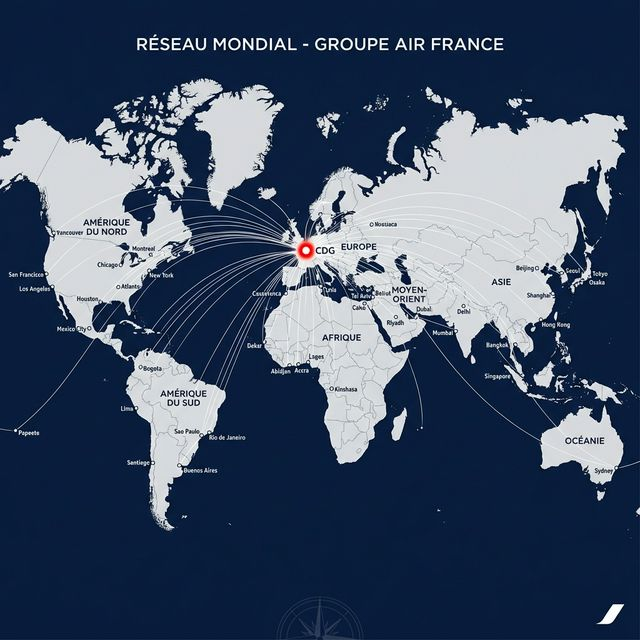
\includegraphics[width=0.65\textwidth]{map_world.png}
\end{center}

\vspace{0.5cm}

\begin{multicols}{2}
\begin{center}
\textbf{\color{eurblue} Réseau Europe}
\vspace{0.2cm}

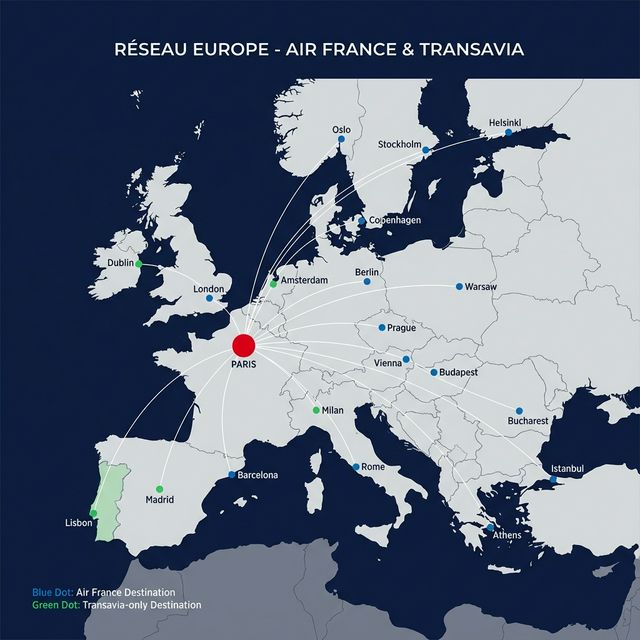
\includegraphics[width=0.95\linewidth]{map_europe.png}
\end{center}

\columnbreak

\begin{center}
\textbf{\color{afrgreen} Réseau Afrique}
\vspace{0.2cm}

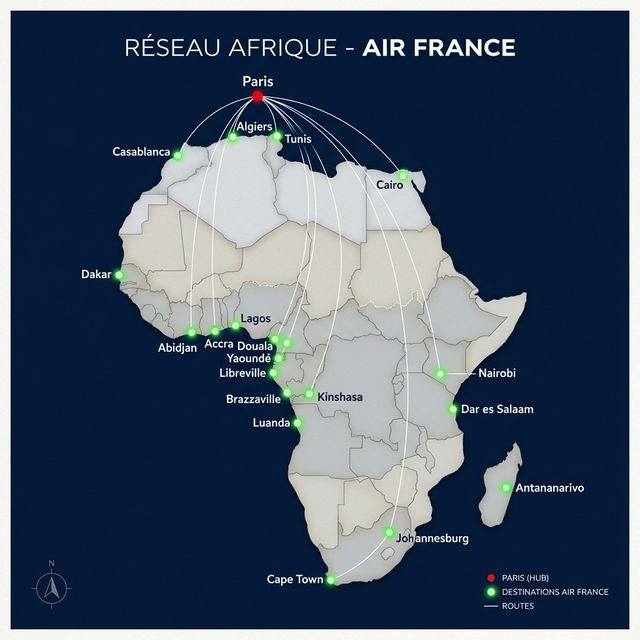
\includegraphics[width=0.95\linewidth]{map_africa.png}
\end{center}
\end{multicols}

\vspace{0.3cm}

\begin{multicols}{2}
\begin{center}
\textbf{\color{asired} Réseau Asie \& Moyen-Orient}
\vspace{0.2cm}

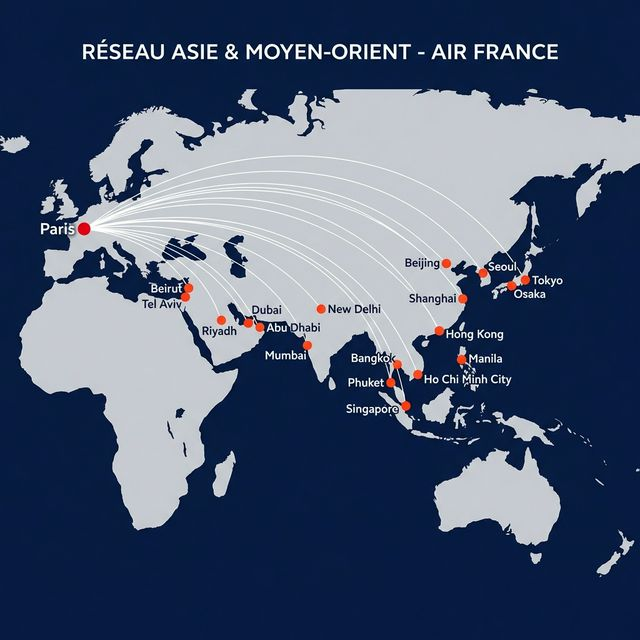
\includegraphics[width=0.95\linewidth]{map_asia.png}
\end{center}

\columnbreak

\begin{center}
\textbf{\color{ameror} Réseau Amériques}
\vspace{0.2cm}

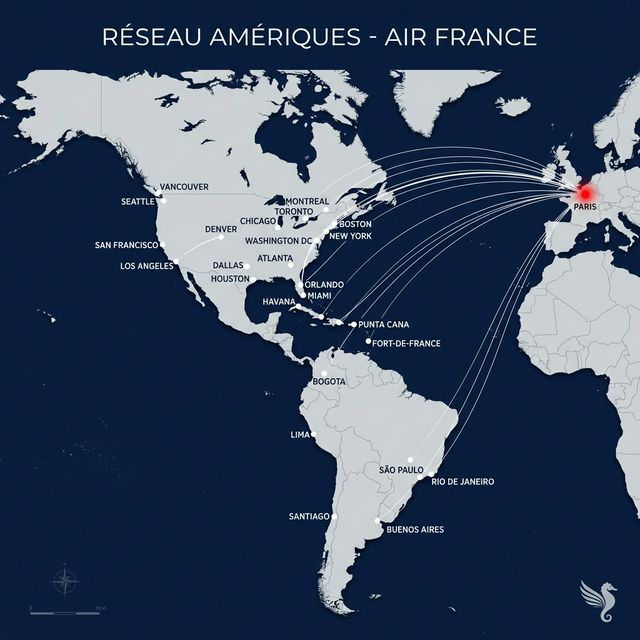
\includegraphics[width=0.95\linewidth]{map_americas.png}
\end{center}
\end{multicols}

\newpage
% ============ DÉCODEUR PRÉFIXES OACI ===================
\sectionbanner{afblue}{DÉCODEUR PRÉFIXES OACI --- À CONNAÎTRE}
\addcontentsline{toc}{section}{Décodeur Préfixes OACI}
\vspace{-0.1cm}

\begin{tcolorbox}[colback=aflight,colframe=afblue,title={\textbf{Comment lire un code OACI ?}},fonttitle=\bfseries\color{white}]
\scriptsize
Un code OACI a \textbf{4 lettres}. La \textbf{1\up{re}} lettre = la \textbf{région du monde}. La \textbf{2\up{e}} lettre = le \textbf{pays} (sauf L et E). Les 2 dernières = l'aéroport spécifique.\\
Exemple : \textbf{LFPG} $\rightarrow$ L (Europe Sud) + F (France) + PG (Paris Charles de Gaulle)
\end{tcolorbox}

\vspace{0.15cm}

\begin{multicols}{3}
\scriptsize

\textbf{\color{afblue}1\up{re} lettre --- Région du monde}\\[-0.1cm]
\begin{tabular}{cl}
\toprule
\textbf{Lettre} & \textbf{Région} \\
\midrule
\rowcolor{eurlight} \textbf{L} & Europe Sud (France, Italie, Espagne\ldots) \\
\textbf{E} & Europe Nord (UK, Pays-Bas, Allemagne\ldots) \\
\rowcolor{eurlight} \textbf{B} & Islande, Groenland \\
\textbf{D} & Afrique de l'Ouest \\
\rowcolor{afrlight} \textbf{F} & Afrique Centre/Sud/Est \\
\textbf{G} & Afrique NO + Golfe de Guinée \\
\rowcolor{afrlight} \textbf{H} & Afrique de l'Est (Kenya, Tanzanie\ldots) \\
\textbf{K} & États-Unis (continentaux) \\
\rowcolor{amerlight} \textbf{C} & Canada \\
\textbf{M} & Amérique Centrale \& Mexique \\
\rowcolor{amerlight} \textbf{S} & Amérique du Sud \\
\textbf{T} & Caraïbes \\
\rowcolor{asilight} \textbf{O} & Moyen-Orient \\
\textbf{V} & Asie du Sud \& Sud-Est \\
\rowcolor{asilight} \textbf{R} & Asie de l'Est (Japon, Corée) \\
\textbf{Z} & Chine \\
\rowcolor{asilight} \textbf{W} & Indonésie, Malaisie \\
\textbf{N} & Pacifique Sud \\
\bottomrule
\end{tabular}

\vspace{0.15cm}
\textbf{\color{afblue}2\up{e} lettre --- Pays (zone L)}\\[-0.1cm]
\begin{tabular}{cl}
\toprule
\textbf{LF} & \textbf{France} \\
\midrule
\rowcolor{eurlight} LI & Italie \\
LE & Espagne \\
\rowcolor{eurlight} LP & Portugal \\
LG & Grèce \\
\rowcolor{eurlight} LH & Hongrie \\
LK & République tchèque \\
\rowcolor{eurlight} LJ & Slovénie \\
LO & Autriche \\
\rowcolor{eurlight} LR & Roumanie \\
LS & Suisse \\
\rowcolor{eurlight} LT & Turquie \\
LY & Serbie \\
\rowcolor{eurlight} LC & Chypre \\
LM & Malte \\
\bottomrule
\end{tabular}

\vspace{0.15cm}
\textbf{\color{afblue}2\up{e} lettre --- Pays (zone E/D/G/autres)}\\[-0.1cm]
\begin{tabular}{cl}
\toprule
\rowcolor{eurlight} \textbf{ED} & Allemagne \\
\textbf{EG} & Royaume-Uni \\
\rowcolor{eurlight} \textbf{EH} & Pays-Bas \\
\textbf{EI} & Irlande \\
\rowcolor{eurlight} \textbf{EK} & Danemark \\
\textbf{EN} & Norvège \\
\rowcolor{eurlight} \textbf{EP} & Pologne \\
\textbf{ES} & Suède \\
\rowcolor{eurlight} \textbf{EF} & Finlande \\
\textbf{EB} & Belgique \\
\midrule
\rowcolor{afrlight} \textbf{DA} & Algérie \\
\textbf{DT} & Tunisie \\
\rowcolor{afrlight} \textbf{GM} & Maroc \\
\textbf{HE} & Égypte \\
\bottomrule
\end{tabular}

\end{multicols}

\begin{tcolorbox}[colback=capgold!10,colframe=capgold!80!black,title={\textbf{$\bigstar$ Moyens mnémotechniques}},fonttitle=\bfseries]
\scriptsize
\begin{multicols}{2}
\begin{itemize}\setlength\itemsep{1pt}
\item \textbf{LF}PG = \textbf{L}a \textbf{F}rance $\rightarrow$ tous les aéroports français commencent par LF
\item \textbf{K} = USA $\rightarrow$ ``\textbf{K}ennedy'' (JFK = KJFK)
\item \textbf{C}Y = \textbf{C}anada $\rightarrow$ Montréal = CYUL
\item \textbf{EG} = \textbf{E}n\textbf{G}lande $\rightarrow$ Londres = EGLL
\item \textbf{ED} = \textbf{E}\textbf{D}eutschland $\rightarrow$ Berlin = EDDB
\item \textbf{LE} = L'\textbf{E}spagne $\rightarrow$ Madrid = LEMD
\item \textbf{LI} = L'\textbf{I}talie $\rightarrow$ Rome = LIRF
\item \textbf{GM} = ``G'Maroc'' $\rightarrow$ Casablanca = GMMN
\item \textbf{DA} = ``D'Algérie'' $\rightarrow$ Alger = DAAG
\item Tous les USA commencent par \textbf{K} sauf Alaska, Hawaï
\end{itemize}
\end{multicols}
\end{tcolorbox}

% ============ AVIONS PAR RÉGION ========================
\newpage
\sectionbanner{afblue}{FLOTTE DÉPLOYÉE PAR RÉGION}
\addcontentsline{toc}{section}{Flotte Déployée par Région}

\begin{multicols}{2}
\scriptsize

\begin{tcolorbox}[colback=eurlight,colframe=eurblue,title={\textbf{COURT \& MOYEN-COURRIER (Europe, Afrique N.)}},fonttitle=\bfseries\color{white}]
\begin{tabular}{lll}
\toprule
\textbf{Avion} & \textbf{Sièges} & \textbf{Routes typiques} \\
\midrule
\textbf{A220-300} & 148 & Florence, Milan, Berlin \\
\textbf{A320} & 174 & Marrakech, Barcelone \\
\textbf{A321} & 212 & Londres, Alger, Istanbul \\
\textbf{A318/319} & 131/143 & Bruxelles, Nice \\
\textbf{Embraer 170/190} & 76/100 & Caen, Strasbourg (HOP) \\
\bottomrule
\end{tabular}\\[0.1cm]
\textit{Cabine : Economy + Business (classe européenne)}\\
\textit{Rayon d'action : jusqu'à $\sim$6\,000 km}
\end{tcolorbox}

\begin{tcolorbox}[colback=asilight,colframe=asired,title={\textbf{LONG-COURRIER}},fonttitle=\bfseries\color{white}]
\begin{tabular}{lll}
\toprule
\textbf{Avion} & \textbf{Sièges} & \textbf{Routes typiques} \\
\midrule
\textbf{A350-900} & 324 & Tokyo, Nairobi, New York \\
\textbf{B777-200ER} & 312 & Dubaï, Abidjan, São Paulo \\
\textbf{B777-300ER} & 468 & New York, Los Angeles \\
\textbf{B787-9} & 276 & Phoenix, Dallas, Le Cap \\
\textbf{A330-200} & 224 & Dakar, Antananarivo \\
\bottomrule
\end{tabular}\\[0.1cm]
\textit{Cabine : La Première / Business / Premium Eco / Economy}\\
\textit{L'A350-900 est le 1\up{er} avion certifié \textbf{ETOPS-370}}
\end{tcolorbox}

\vspace{0.15cm}

\begin{tcolorbox}[colback=amerlight,colframe=ameror,title={\textbf{TRANSAVIA (TO)}},fonttitle=\bfseries\color{white}]
\begin{tabular}{lll}
\toprule
\textbf{Avion} & \textbf{Sièges} & \textbf{Routes typiques} \\
\midrule
\textbf{B737-800} & 189 & Marrakech, Porto, Athènes \\
\textbf{B737 MAX 8} & 189 & Tenerife, Dubaï \\
\bottomrule
\end{tabular}\\[0.1cm]
\textit{Cabine : classe unique (Economy). Flotte 100\% Boeing.}
\end{tcolorbox}

\end{multicols}

% ============ HUBS PARIS ===============================
\sectionbanner{afblue}{HUBS PARIS --- CDG \& ORLY}
\addcontentsline{toc}{section}{Hubs Paris}

\begin{multicols}{2}
\scriptsize

\begin{tcolorbox}[colback=aflight,colframe=afblue,title={\textbf{PARIS-CHARLES DE GAULLE (CDG / LFPG)}},fonttitle=\bfseries\color{white}]
\begin{tabular}{rl}
\textbf{Ouverture} & 1974 \\
\textbf{Pistes} & 4 (dont 2 de 4\,215 m) \\
\textbf{Terminaux AF} & 2E, 2F, 2G \\
\textbf{Passagers} & $\sim$70 M/an (\#1 France, \#2 Europe) \\
\textbf{Vocation} & Hub principal AF, tous long-courriers \\
\textbf{Correspondances} & Min. 1h (interligne), 45 min (même cie) \\
\end{tabular}
\end{tcolorbox}

\begin{tcolorbox}[colback=aflight,colframe=afred,title={\textbf{PARIS-ORLY (ORY / LFPO)}},fonttitle=\bfseries\color{white}]
\begin{tabular}{rl}
\textbf{Ouverture} & 1932 (principal jusqu'en 1974) \\
\textbf{Pistes} & 3 \\
\textbf{Terminaux AF} & Orly 1 \\
\textbf{Passagers} & $\sim$33 M/an (\#2 France) \\
\textbf{Vocation} & Domestique + Outre-mer + Transavia \\
\textbf{Note 2026} & AF se retire d'Orly (tout vers CDG) \\
\end{tabular}
\end{tcolorbox}

\end{multicols}

% ============ SKYTEAM ================================
\sectionbanner{eurblue}{HUBS SKYTEAM --- RÉSEAU PARTENAIRES}
\addcontentsline{toc}{section}{Hubs SkyTeam}

\begin{tcolorbox}[colback=eurlight,colframe=afblue,title={\textbf{Les 19 membres SkyTeam et leurs hubs principaux}},fonttitle=\bfseries\color{white}]
\scriptsize
\begin{multicols}{3}
\begin{tabular}{lll}
\toprule
\textbf{Compagnie} & \textbf{Hub} & \textbf{IATA} \\
\midrule
\rowcolor{aflight} Air France & Paris CDG & CDG \\
KLM & Amsterdam & AMS \\
\rowcolor{aflight} Delta & Atlanta & ATL \\
Korean Air & Séoul & ICN \\
\rowcolor{aflight} Aeromexico & Mexico & MEX \\
Aeroflot & Moscou & SVO \\
\rowcolor{aflight} China Eastern & Shanghai & PVG \\
Vietnam Airlines & Hanoï & HAN \\
\rowcolor{aflight} Saudi Arabian & Djeddah & JED \\
Garuda Indonesia & Jakarta & CGK \\
\rowcolor{aflight} China Airlines & Taipei & TPE \\
ITA Airways & Rome & FCO \\
\rowcolor{aflight} Czech Airlines & Prague & PRG \\
Tarom & Bucarest & OTP \\
\rowcolor{aflight} Middle East Al. & Beyrouth & BEY \\
Kenya Airways & Nairobi & NBO \\
\rowcolor{aflight} XiamenAir & Xiamen & XMN \\
Aerolíneas Arg. & Buenos Aires & EZE \\
\rowcolor{aflight} SAS & Copenhague & CPH \\
\bottomrule
\end{tabular}
\end{multicols}
\end{tcolorbox}

% ============ TOP ROUTES ==============================
\sectionbanner{afred}{TOP 15 ROUTES AIR FRANCE}
\addcontentsline{toc}{section}{Top 15 Routes}

\begin{multicols}{2}
\scriptsize
\begin{tabular}{clccc}
\toprule
\textbf{\#} & \textbf{Route} & \textbf{Fréq/sem} & \textbf{Avion} & \textbf{Vol} \\
\midrule
\rowcolor{aflight} 1 & CDG -- JFK (New York) & 49 (7/j) & B777-300ER & 8h15 \\
2 & CDG -- LHR (Londres) & 35 (5/j) & A320/A321 & 1h15 \\
\rowcolor{aflight} 3 & CDG -- AMS (Amsterdam) & 28 (4/j) & A220/A320 & 1h15 \\
4 & CDG -- ABJ (Abidjan) & 14 (2/j) & B777/A350 & 6h25 \\
\rowcolor{aflight} 5 & CDG -- HND (Tokyo) & 14 (2/j) & B777-300ER & 12h \\
6 & CDG -- DXB (Dubaï) & 14 (2/j) & A350-900 & 6h30 \\
\rowcolor{aflight} 7 & CDG -- BKK (Bangkok) & 13 & A350-900 & 11h15 \\
8 & CDG -- CMN (Casablanca) & 14 & A321/B777 & 3h05 \\
\rowcolor{aflight} 9 & ORY -- FDF (Fort-de-Fr.) & 14 (2/j) & B777-300ER & 8h30 \\
10 & CDG -- SIN (Singapour) & 10 & A350-900 & 12h30 \\
\rowcolor{aflight} 11 & CDG -- LAX (Los Angeles) & 14 (2/j) & B777-200ER & 11h15 \\
12 & CDG -- FCO (Rome) & 35 (5/j) & A220/A320 & 2h10 \\
\rowcolor{aflight} 13 & CDG -- BCN (Barcelone) & 28 (4/j) & A220/A320 & 1h50 \\
14 & CDG -- GRU (São Paulo) & 10 & B777-300ER & 11h30 \\
\rowcolor{aflight} 15 & CDG -- YUL (Montréal) & 14 (2/j) & A350/B787 & 7h30 \\
\bottomrule
\end{tabular}
\end{multicols}

% ============ QCM DESTINATIONS ========================
\newpage
\sectionbanner{afrgreen}{QCM --- DESTINATIONS \& CODES (15 questions)}
\addcontentsline{toc}{section}{QCM Destinations}

\begin{multicols}{2}
\scriptsize

\textbf{Q1.} Quel est le code OACI de Paris CDG ?\\
a) LFPO \quad b) LFPG \quad c) LFOB \quad d) EDDF

\textbf{Q2.} Le préfixe OACI ``K'' correspond à quel pays ?\\
a) Canada \quad b) Kenya \quad c) États-Unis \quad d) Corée du Sud

\textbf{Q3.} Combien de destinations AF dessert-elle environ ?\\
a) 100 \quad b) 150 \quad c) 200 \quad d) 300

\textbf{Q4.} Quel est le code IATA de Tokyo Haneda ?\\
a) NRT \quad b) TYO \quad c) HND \quad d) KIX

\textbf{Q5.} Le code OACI ``KJFK'' correspond à :  \\
a) Jakarta \quad b) Johannesburg \quad c) New York JFK \quad d) Jeddah

\textbf{Q6.} Quelle est la destination la plus fréquente au départ de CDG ?\\
a) Londres \quad b) New York JFK \quad c) Dubaï \quad d) Tokyo

\textbf{Q7.} Le code IATA ``DSS'' correspond à :  \\
a) Dallas \quad b) Dakar \quad c) Djibouti \quad d) Dar es Salaam

\textbf{Q8.} Quel avion est déployé en priorité sur Tokyo et New York ?\\
a) A350-900 \quad b) A320neo \quad c) B777-300ER \quad d) B787-9

\textbf{Q9.} Le préfixe OACI ``DA'' correspond à quel pays ?\\
a) Danemark \quad b) Algérie \quad c) Allemagne \quad d) Djibouti

\textbf{Q10.} Quelle est la durée approximative d'un vol CDG--Singapour ?\\
a) 8h30 \quad b) 10h00 \quad c) 12h30 \quad d) 15h00

\textbf{Q11.} Quel est le 2\up{e} aéroport parisien après CDG ?\\
a) Le Bourget \quad b) Beauvais \quad c) Orly \quad d) Villacoublay

\textbf{Q12.} Air France fait partie de quelle alliance ?\\
a) Star Alliance \quad b) Oneworld \quad c) SkyTeam \quad d) Aucune

\textbf{Q13.} Le code IATA de Montréal est :  \\
a) YYZ \quad b) YVR \quad c) YUL \quad d) YQB

\textbf{Q14.} Transavia utilise principalement quel type d'avion ?\\
a) A220-300 \quad b) B737-800 \quad c) A320neo \quad d) Embraer 190

\textbf{Q15.} Combien de pistes Paris CDG possède-t-il~?\\
a) 2 \quad b) 3 \quad c) 4 \quad d) 5

\vspace{0.3cm}
\begin{tcolorbox}[colback=afrlight,colframe=afrgreen,title={\textbf{CORRIGÉS}},fonttitle=\bfseries\color{white}]
\begin{tabular}{cccccccc}
Q1 & Q2 & Q3 & Q4 & Q5 & Q6 & Q7 & Q8 \\
b & c & c & c & c & b & b & c \\
\midrule
Q9 & Q10 & Q11 & Q12 & Q13 & Q14 & Q15 & \\
b & c & c & c & c & b & c & \\
\end{tabular}
\end{tcolorbox}

\end{multicols}

% ============ STATISTIQUES ============================
\vspace{0.3cm}
\begin{tcolorbox}[colback=aflight,colframe=afblue,title={\textbf{STATISTIQUES RÉSEAU --- À RETENIR POUR LE PSY0}},fonttitle=\bfseries\color{white}]
\begin{multicols}{3}
\scriptsize
\begin{itemize}\setlength\itemsep{0pt}
\item[\textbf{$\sim$200}] destinations totales
\item[\textbf{$\sim$80}] pays desservis
\item[\textbf{19}] villes aux USA
\item[\textbf{5}] villes au Canada
\item[\textbf{14}] aéroports en Italie
\item[\textbf{9}] villes au Maroc
\item[\textbf{14}] villes en Espagne
\item[\textbf{7}] villes en Algérie
\item[\textbf{22}] pays en Afrique subsah.
\item[\textbf{14}] destinations en Asie-Pac.
\item[\textbf{25}] villes France métro
\item[\textbf{4}] territoires outre-mer
\item Vol le plus court : CDG--BRU (\textbf{1h05})
\item Vol le plus long : CDG--PPT (\textbf{$\sim$21h} via LAX)
\item Hub principal : \textbf{CDG} (T2E/F/G)
\item Code OACI France : \textbf{LF}
\item Code OACI USA : \textbf{K}
\item Alliance : \textbf{SkyTeam} (19 membres)
\end{itemize}
\end{multicols}
\end{tcolorbox}

\vfill
\begin{center}
\rule{0.6\textwidth}{0.5pt}\\[0.15cm]
{\scriptsize Sources : Air France Corporate 2025, Transavia.com, Wikipedia, FlightConnections, programmes hiver 2025-2026 et été 2025.}\\
{\scriptsize Distances et durées approximatives. Certaines destinations sont saisonnières. \CAP\ = Capitale du pays.}\\[0.15cm]
{\small\textbf{Document préparé pour la révision PSY0 Cadets Air France --- Février 2026}}
\end{center}

\end{document}
